\documentclass[a4paper, 12pt]{article}
\usepackage[utf8]{inputenc}
\usepackage[T1]{fontenc}
\usepackage[french]{babel}
\usepackage{graphicx}
\usepackage{amsmath}
\usepackage{hyperref}
\usepackage{lmodern}
\usepackage{moreverb}
\usepackage{multicol}

\hypersetup{
    colorlinks=true,
    linkcolor=blue,
    filecolor=magenta,      
    urlcolor=cyan,
    pdftitle={Overleaf Example},
    pdfpagemode=FullScreen,
    }

\urlstyle{same}
\usepackage[a4paper,left=2cm,right=2cm,top=2cm,bottom=2cm]{geometry}

\pagestyle{headings}
\pagestyle{plain}


\setcounter{secnumdepth}{4}
\setcounter{tocdepth}{4}
\makeatletter


\makeatother



\makeatletter
\def\toclevel@subsubsubsection{4}
\def\toclevel@paragraph{5}
\def\toclevel@subparagraph{6}
\makeatother





\setlength{\parindent}{0cm}
\setlength{\parskip}{1ex plus 0.5ex minus 0.2ex}
\newcommand{\hsp}{\hspace{20pt}}
\newcommand{\HRule}{\rule{\linewidth}{0.5mm}}

\begin{document}

\begin{titlepage}
  \begin{sffamily}
  \begin{center}

   
    \textsc{\LARGE }\\[2cm]

    \textsc{\Large Compte rendu de Réunion}\\[1.5cm]
    \textsc{\Medium Rédigé par ZEGHDALLOU Ilyes}

    % Title
    \HRule \\[0.4cm]
    { \huge  \textsc{StellaStone} \\
    \textsc{\Large By Novus}\\ [0.4cm] }
	

    \HRule \\[2cm]
    \textsc {Idriss BENGUEZZOU\\Mohammed ROUABAH\\Ghilas MEZIANE \\ Ilyes ZEGHDALLOU}
 \begin{figure}
     \centering
    
\includegraphics[scale=0.2]{logoUJM.png}
     \label{fig:ujm_logo}
 \end{figure}
   
    \

    \vfill

    % Bottom of the page
    {\large {} 11/11/2022}

  \end{center}
  \end{sffamily}
\end{titlepage}

\newpage

\section{Réunion du Vendredi 11/11}
La réunion de cette semaine a eu lieu le vendredi 11 novembre 2022, en distanciel - étant donné que c'était un jour férié - sur notre serveur DISCORD, sur le créneau horaire 17h-18h.

\textbf{Ordre du jour :}
 \begin{itemize}
     \item Révision du document de spécification des exigences.
     \item Révision du document test des recettes.
     \item Introduction au document de conception générale.
 \end{itemize}
\section{Tour de table habituel}
Nous avons débuté la réunion par un bref tour de table afin de permettre à chacun d'énumérer les parties qu'il a rédigé et une estimation de son avancement, et ce dans le but de nous situer avant de passer à la révision et la relecture des documents. \\

Mr.ROUABAH Mohammed a annoncé avoir terminé les exigences fonctionnelles de la partie profil. \\
Mr.MEZIANE Ghilas nous a fait savoir que les exigences fonctionnelles concernant la partie du Réseau spatial seraient achevées durant la semaine.\\
Mr.BENGUEZZOU Idriss a ensuite fait part de son avancement concernant les exigences fonctionnelles de la partie Entreprise, qu'il a estimé à 80\%. \\
Enfin Mr.ZEGHDALLOU Ilyes a exprimé son inquiétude concernant le document de tests de recette qui -pour lui- prenait peut être du retard.\\
Mr.MEZIANE Ghilas, a fait remarquer à l'ensemble des membres de la société Novus que certaines dates butoirs risquaient de ne pas être respectées. C'est pourquoi en plus des objectifs prévus pour la réunion du jour, Nous avons consacré un moment pour redéfinir notre calendrier.

\section{Révision du planning}
Nous avons opté pour une modification des dates butoirs ce qui engendre une modification de notre diagramme de Gantt.
Ainsi, les décisions prises sont les suivantes :

\begin{enumerate}
    \item Repousser la date de début de rédaction du document de conception générale au 11/11/2022 (Ex-date: 30/10/2022).\\
    \item La décision précédente engendre une modification de la date de début de rédaction du document des tests d'intégration au 18/11/2022. \\
    \item Avancer la date de début de conception des maquettes Figma au 11/11/2022.
\end{enumerate}

 \begin{figure}[!h]
    \centering
    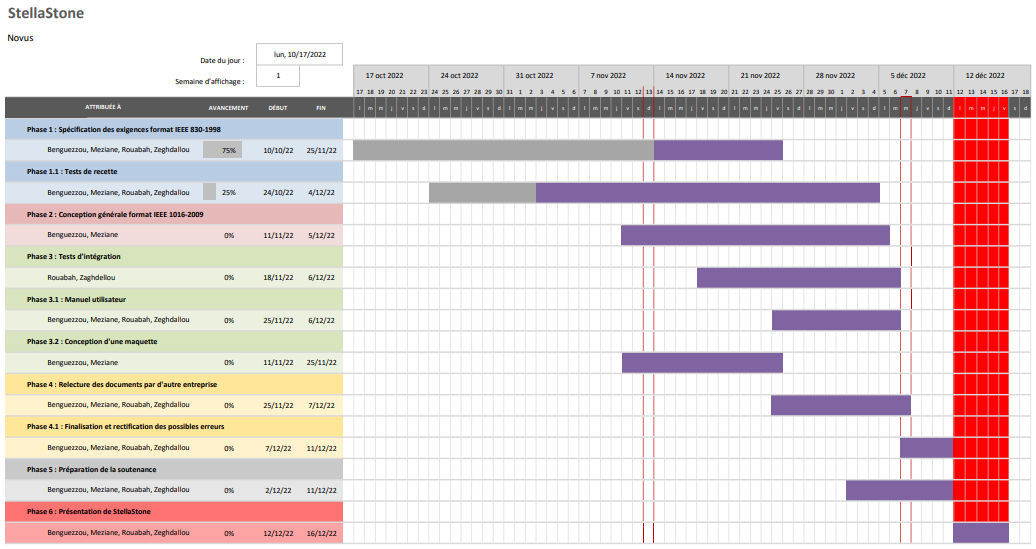
\includegraphics[scale=0.4648]{Diagramme de gantt.png}
    \label{fig:Le_planning}
    \caption{Nouvelle date du planning}
\end{figure}

\newpage
\subsection{Relecture des documents}
Après une correction orthographique, nous avons revus ensemble l'aspect lexicographique de notre document de spécification des exigences.
Nous avons notamment unifié les formats pour l'énumération de nos exigences: \\
\begin{itemize}
\item EI-XXX-...-N pour les exigences des interfaces externes.\\
\item EF-XXX-...-N pour les exigences fonctionnelles.\\
\item EP-XXX-...-N pour les exigences de performance.\\
\item EBD-XXX-...-N pour les exigences relatives à la base de données.
\end{itemize}


\section{Prochaine réunion et objectifs de la semaine}
Comme objectifs de la semaine, Mr.BENGUEZZOU et Mr.MEZIANE continueront la rédaction des exigences fonctionnelles, et entameront la réalisation de la maquette sur FIGMA.
Mr.ROUABAH et Mr.ZEGHDALLOU commenceront la rédaction du document de conception générale, et poursuivront la rédaction du document de tests de recette. 
La prochaine réunion est fixée pour le vendredi 18 novembre 2022, sur le créneau horaire 17h-18h avec pour ordre du jour: \\

\begin{itemize}
    \item Révision du document de spécification des exigences.
    \item Révision du document de tests de recette.
    \item Observation de l'avancement du document de conception générale. \\
\end{itemize}

La prochaine personne en charge de la rédaction du compte rendu de réunion est : MEZIANE Ghilas.

\end{document}